%
% ellintegral.tex
%
% (c) 2021 Prof Dr Andreas Müller, OST Ostschweizer Fachhochschule
%
\section{Elliptische Integrale
\label{buch:elliptisch:section:integral}}
\rhead{Elliptisches Integral}
Bei der Berechnung des Ellipsenbogens in 
Abschnitt~\ref{buch:geometrie:subsection:kegelschnitte}
sind wir auf ein Integral gestossen, welches sich nicht in geschlossener
Form ausdrücken liess.
Um solche Integrale in den Griff zu bekommen, ist es nötig, sie als
neue spezielle Funktionen zu definieren.

\subsection{Definition
\label{buch:elliptisch:subsection:definition}}
Ein {\em elliptisches Integral} ist ein Integral der Form
\index{elliptisches Integral}%
\index{Integral, elliptisch}%
\begin{equation}
\int R\left( x, \sqrt{p(x)}\right)\,dx
\label{buch:elliptisch:def:allgemein}
\end{equation}
wobei $R(x,y)$ eine rationale Funktion von zwei Variablen ist und
$p(x)$ ein Polynom dritten oder vierten Grades.
Hätte $p(x)$ ein mehrfache Nullstelle $x_0$, müsste es durch $(x-x_0)^2$
teilbar sein, man könnte also einen Faktor $(x-x_0)$ aus der
Wurzel im Integraneden von \eqref{buch:elliptisch:def:allgemein}
ausklammern und damit das Integral in eine Form bringen, wo $p(x)$
höchstens zweiten Grades ist.
Solche Integrale lassen sich meistens mit trigonometrischen Substitutionen
berechnen.
Wir verlangen daher, dass $p(x)$ keine mehrfachen Nullstellen hat.

Man kann zeigen, dass sich elliptische Integrale in Summen von
elementaren Funktionen und speziellen elliptischen Integralen 
der folgenden Form überführen lassen
\cite[Abschnitt 164, p.~506]{buch:smirnov32}.

\begin{definition}
\label{buch:elliptisch:def:integrale123}
Die elliptischen Integrale erster, zweiter und dritter Art sind die
Integrale
\[
\begin{aligned}
\text{1.~Art:}&&&
\int \frac{dx}{\sqrt{(1-x^2)(1-k^2x^2)}}
\\
\text{2.~Art:}&&&
\int \sqrt{\frac{1-k^2x^2}{1-x^2}}\,dx
\\
\text{3.~Art:}&&&
\int \frac{dx}{(1-nx^2)\sqrt{(1-x^2)(1-k^2x^2)}}
\end{aligned}
\]
mit $0<k<1$.
Es ist auch üblich, den Parameter $m=k^2$ zu verwenden.
Die Zahl $k$ heisst {\em Modul} des elliptischen Integrals.
\index{Modul eines elliptischen Integrals}%
\index{elliptisches Integral}%
\end{definition}

Wie gesagt lassen sich für diese unbestimmten Integrale keine 
geschlossenen Formen finden.
Es bleibt uns daher nichts anderes übrig, als die Integralgrenzen
festzulegen und damit eine Stammfunktion auszuwählen.

%
% Elliptisches Integral
%
\subsection{Vollständige elliptische Integrale
\label{buch:elliptisch:subsection:vollstaendig}}
In diesem Abschnitt legen wir beide Integrationsgrenzen fest und
untersuchen die entstehenenden Funktionen von den Parametern
$k$ und $n$.

\subsubsection{Definition der vollständigen elliptischen Integrale}
Da der Nenner in allen drei elliptischen Integralen eine Nullstelle
bei $\pm1$ hat, kann das Integral nur von $0$ bis $1$ erstreckt werden.

\begin{definition}
\label{buch:elliptisch:def:vollstintegrale123}
Die vollständigen elliptischen Integrale erster, zweiter und dritter
Art sind
\[
\begin{aligned}
\text{1.~Art:}&&
K(k)&=\int_0^1 \frac{dt}{\sqrt{(1-t^2)(1-k^2t^2)}} \\
\text{2.~Art:}&&
E(k)&=\int_0^1 \sqrt{\frac{1-k^2t^2}{1-t^2}}\,dt \\
\text{3.~Art:}&&
\Pi(n, k)&=\int_0^1\frac{dt}{(1-nt^2)\sqrt{(1-t^2)(1-k^2t^2)}} 
\end{aligned}
\]
mit $0<k<1$.
\end{definition}

Die Funktionen hängen stetig von $k$ ab.
Die Nullstellen des Faktors $1-k^2x^2$ liegen ausserhalb des
Integrationsintervalls und spielen daher keine Rolle.
Die Werte von $K(k)$ und $E(k)$ für $k=0$ können direkt berechnet
werden:
\begin{align*}
K(0)
=
E(0)
&=
\int_0^1 \frac{dt}{\sqrt{1-t^2}}=\frac{\pi}2.
\end{align*}
Das Integral $\Pi(n,0)$ ist etwas komplizierter.

Für $k\to 1$ ist $E(k)=1$, die Integrale $K(1)$ und $\Pi(n,1)$
sind dagegen divergent.

\subsubsection{Jacobi- und Legendre-Normalform}
Die Integrationsvariable $t$ der vollständigen elliptischen Integrale
kann durch die Substitution $t=\sin\varphi$ durch die Variable
$\varphi$ und das Integral über das Intervall $[0,1]$ durch ein
Integral über das Intervall $[0,\frac{\pi}2]$ ersetzt werden.
Mit
\[
\frac{dt}{d\varphi} = \cos\varphi = \sqrt{1-\sin^2\varphi}
\]
können die Funktionen $K(k)$, $E(k)$ und $\Pi(n,k)$ auch als
\begin{align*}
K(k)
&=
\int_0^{\frac{\pi}2}
\frac{
\sqrt{1-\sin^2\varphi}\,d\varphi
}{
\sqrt{(1-\sin^2\varphi)(1-k^2\sin^2\varphi)}
}
=
\int_0^{\frac{\pi}2}
\frac{d\varphi}{\sqrt{1-k^2\sin^2\varphi}}
,
\\
E(k)
&=
\int_0^{\frac{\pi}2}
\sqrt{\frac{1-k^2\sin^2\varphi}{1-\sin^2\varphi}}\sqrt{1-\sin^2\varphi}\,d\varphi
=
\int_0^{\frac{\pi}2}
\sqrt{1-k^2\sin^2\varphi}\,d\varphi
,
\\
\Pi(n,k)
&=
\int_0^{\frac{\pi}2}
\frac{
\sqrt{1-\sin^2\varphi}\,d\varphi
}{
(1-n\sin^2\varphi)\sqrt{(1-\sin^2\varphi)(1-k^2\sin^2\varphi)}
}
=
\int_0^{\frac{\pi}2}
\frac{
d\varphi
}{
(1-n\sin^2\varphi)\sqrt{1-k^2\sin^2\varphi}
}
.
\end{align*}
Diese Form wird auch die {\em Legendre-Normalform} der vollständigen 
\index{Legendre-Normalform}%
elliptischen Integrale genannt, während die Form von
Definition~\ref{buch:elliptisch:def:vollstintegrale123}
die {\em Jacobi-Normalform} heisst.
\index{Jacobi-Normalform}%

\subsubsection{Vollständige elliptische Integrale als hypergeometrische
Funktionen}
%XXX Als hypergeometrische Funktionen \url{https://www.youtube.com/watch?v=j0t1yWrvKmE} \\
Das vollständige elliptische Integral $K(k)$ kann mit Hilfe der 
Binomialreihe umgeformt werden in eine hypergeometrische Reihe.
Da im Integral nur $k^2$ auftaucht, wird sich $K(k)$ als
hypergeometrische Funktion von $k^2$ ausdrücken lassen.

\begin{satz}
\label{buch:elliptisch:satz:hyperK}
Das vollständige elliptische Integral $K(k)$ lässt sich durch die
hypergeometrische Funktion $\mathstrut_2F_1$ als
\[
K(k)
=
\frac{\pi}2
\cdot
\mathstrut_2F_1\biggl(
\begin{matrix}\frac12,\frac12\\1\end{matrix};1;k^2
\biggr)
\]
ausdrücken.
\end{satz}

\begin{proof}[Beweis]
Zunächst ist das vollständige elliptische Integral in der Legendre-Form
\begin{align}
K(k)
&=
\int_0^{\frac{\pi}2}
\frac{d\vartheta}{\sqrt{1-k^2\sin^2\vartheta}}
%\notag
%\\
%&
=
\int_0^{\frac{\pi}2}
\bigl(
1-(k\sin\vartheta)^2
\bigr)^{-\frac12}\,d\vartheta.
\notag
\intertext{Die Wurzel im letzten Integral kann mit Hilfe der binomischen
Reihe vereinfacht werden zu}
&=
\sum_{n=0}^\infty
(-1)^n k^2\binom{-\frac12}{n}
\int_0^{\frac{\pi}2}
\sin^{2n}\vartheta
\,d\vartheta.
\label{buch:elliptisch:beweis:ellharm2}
\end{align}
Der verallgemeinerte Binomialkoeffizient lässt sich nach
\begin{align*}
\binom{-\frac12}{n}
&=
\frac{(-\frac12)(-\frac32)(-\frac52)\cdot\ldots\cdot(-\frac12-n+1)}{n!}
=
(-1)^n
\cdot
\frac{1}{n!}
\cdot
\frac12\cdot\frac32\cdot\frac52\cdot\ldots\cdot\biggl(\frac12+n-1\biggr)
=
(-1)^n\frac{(\frac12)_n}{n!}
\end{align*}
vereinfachen.
Setzt man dies in \eqref{buch:elliptisch:beweis:ellharm2} ein, erhält
man
\begin{align*}
K(k)
&=
\sum_{n=0}^\infty
(-1)^n k^{2n}
\cdot
(-1)^n
\frac{(\frac12)_n}{n!}
\cdot
\int_0^{\frac{\pi}2} \sin^{2n}\vartheta\,d\vartheta
=
\sum_{n=0}^\infty
\frac{(\frac12)_n}{n!}
\int_0^{\frac{\pi}2} \sin^{2n}\vartheta\,d\vartheta
\cdot (k^2)^n.
\end{align*}
Es muss jetzt also nur noch das Integral von $\sin^{2n}\vartheta$
berechnet werden.
Mit partieller Integration kann man
\begin{align*}
\int \sin^m\vartheta\,d\vartheta
&=
\int
\underbrace{\sin \vartheta}_{\uparrow}
\underbrace{\sin^{m-1}\vartheta}_{\downarrow}
\,d\vartheta
\\
&=
-\cos\vartheta\sin^{m-1}\vartheta
+
\int \cos^2\vartheta (m-1)\sin^{m-2}\vartheta\,d\vartheta
\\
&=
-\cos\vartheta \sin^{m-1}\vartheta
+
(m-1)
\int
(1-\sin^2\vartheta)
\sin^{m-2}\vartheta\,d\vartheta.
\end{align*}
Wegen $\sin 0=0$ und
$\cos\frac{\pi}2=0$ verschwindet der erste Term im bestimmten Integral
und der zweite wird
\begin{align*}
\int_0^{\frac{\pi}2}
\sin^{m} \vartheta
\,d\vartheta
&=
(m-1)
\int_0^{\frac{\pi}2}
\sin^{m-2}\vartheta\,d\vartheta
-
(m-1)
\int_0^{\frac{\pi}2}
\sin^m \vartheta\,d\vartheta
\\
m
\int_0^{\frac{\pi}2}
\sin^{m} \vartheta\,d\vartheta
&=
(m-1)
\int_0^{\frac{\pi}2}
\sin^{m-2} \vartheta\,d\vartheta
\\
\int_0^{\frac{\pi}2}
\sin^{m} \vartheta\,d\vartheta
&=
\frac{m-1}{m}
\int_0^{\frac{\pi}2}
\sin^{m-2} \vartheta\,d\vartheta.
\end{align*}
Mit dieser Rekursionsformel kann jetzt das Integral berechnet werden.
Es folgt
\begin{align*}
\int_0^{\frac{\pi}2}
\sin^{2n}\vartheta\,d\vartheta
&=
\frac{2n-1}{2n}
\int_0^{\frac{\pi}2}
\sin^{2n-2}\vartheta\,d\vartheta
\\
&=
\frac{2n-1}{2n}
\frac{2n-3}{2n-2}
\frac{2n-5}{2n-4}
\cdots
\frac{2n-(2n-1)}{2(n-1)}
\int_0^{\frac{\pi}2}
\sin^{2n-4}\vartheta\,d\vartheta
\\
&=
\frac{
(n-\frac12)(n-\frac32)(n-\frac52)\cdot\ldots\cdot\frac32\cdot\frac12
}{
n!
}
\int_0^{\frac{\pi}2} 1\,d\vartheta
\\
&=
\frac{(\frac12)_n}{n!}
\cdot
\frac{\pi}2.
\end{align*}
Damit wird die Reihenentwicklung für $K(k)$ jetzt zu
\[
K(k)
=
\frac{\pi}2
\sum_{n=0}^\infty
\frac{(\frac12)_n(\frac12)_n}{n!} \cdot \frac{(k^2)^n}{n!}
=
\frac{\pi}2
\cdot
\mathstrut_2F_1\biggl(\begin{matrix}\frac12,\frac12\\1\end{matrix};k^2\biggr),
\]
dies beweist die Behauptung.
\end{proof}

%
% Umfang einer Ellipse
%
\subsubsection{Umfang einer Ellipse}
\begin{figure}
\centering
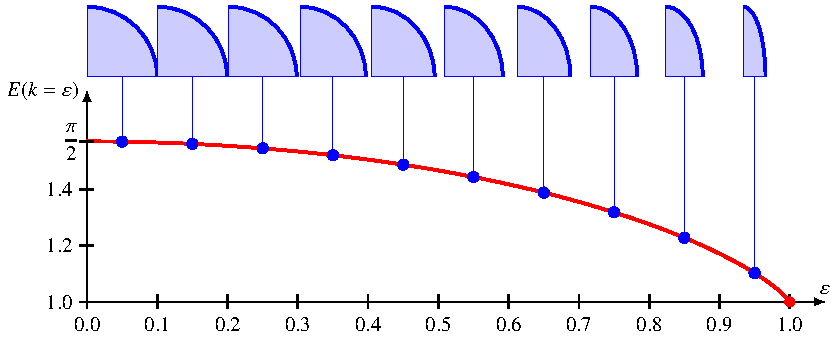
\includegraphics{chapters/110-elliptisch/images/ellipsenumfang.pdf}
\caption{Bogenlänge eines Viertels einer Ellipse mit Exzentrizität
$\varepsilon$.
Eine solche Ellipse hat Halbachsen $1$ und $\sqrt{1-\varepsilon^2}$,
ein entsprechender Ellipsenbogen ist für ausgewählte Werte in blau
eingezeichnet.
\label{buch:elliptisch:fig:ellipsenumfang}}
\end{figure}
Wir zeigen, wie sich die Berechnung des Umfangs $U$ einer Ellipse
mit Halbachsen $a$ und $b$, $a\le b$, auf ein volltändiges elliptisches
Integral zurückführen lässt.
Der Fall $a>b$ kann behandelt werden, indem die $x$- und $y$-Koordinaten
vertauscht werden.

Die Parametrisierung
\[
t\mapsto \begin{pmatrix}a\cos t\\ b\sin t\end{pmatrix}
\]
einer Ellipse führt auf das Integral
\begin{align}
U
&=
\int_0^{2\pi} \sqrt{a^2\sin^2t + b^2\cos^2 t}\,dt
\notag
\\
&=
4\int_0^{\frac{\pi}2}
\sqrt{a^2\sin^2t + b^2(1-\sin^2 t)}
\,dt
\notag
\\
&=
4b \int_0^{\frac{\pi}2} \sqrt{1-(b^2-a^2)/b^2\cdot \sin^2t}\,dt
\label{buch:elliptisch:eqn:umfangellipse}
\end{align}
für den Umfang der Ellipse.
Bei einem Kreis ist $a=b$ und der zweite Term unter der Wurzel fällt weg,
der Umfang wird $4b\frac{\pi}2=2\pi b$.
Die Differenz $e^2=b^2-a^2$ ist die {\em lineare Exzentrizität} der Ellipse,
\index{lineare Exzentrizität}%
der Quotient $e/b$ wird die {\em numerische Exzentrizität} der Ellipse
genannt.
Insbesondere ist $k = \varepsilon$.

Das Integral~\eqref{buch:elliptisch:eqn:umfangellipse} erhält jetzt die
Form
\[
U
=
4b\int_0^{\frac{\pi}2} \sqrt{1-k^2\sin^2t}\,dt
\]
und ist damit als elliptisches Integral zweiter Art erkannt.
Für den Umfang der Ellipse finden wir damit die Formel
\[
U
=
4b E(k)
=
4b E(\varepsilon).
\]
Das vollständige elliptische Integral zweiter Art $E(\varepsilon)$
liefert also genau den Umfang eines Viertels der Ellipse mit
numerischer Exzentrizität $\varepsilon$ und kleiner Halbachse $1$.
Für den extremen Wert $\varepsilon=0$ entsteht der Umfang einer Ellipse,
also $E(0)=\frac{\pi}2$.
Für $\varepsilon=1$ ist $a=0$, es entsteht eine Strecke mit Länge $E(1)=1$.

\begin{satz}
\label{buch:elliptisch:satz:hyperE}
Das volständige elliptische Integral $E(k)$ ist
\[
E(k)
=
\int_0^{\frac{\pi}2} \sqrt{1-k^2\sin^2\vartheta}\,d\vartheta
=
\frac{\pi}2
\cdot
\mathstrut_2F_1\biggl(
\begin{matrix}-\frac12,\frac12\\1\end{matrix};
k^2
\biggr).
\]
\end{satz}

\begin{proof}[Beweis]
Die Identität kann wie im Satz~\ref{buch:elliptisch:satz:hyperK} mit
Hilfe einer Entwicklung der Wurzel mit der Binomialreihe gefunden
werden.
\end{proof}

Die Darstellung von $E(k)$ als hypergeometrische Reihe ermöglicht
jetzt zum Beispiel auch die Berechnung der Ableitung nach dem
Parameter $k$ mit der Ableitungsformel für die Funktion $\mathstrut_2F_1$.


%
% Berechnung mit dem arithmetisch-geometrischen Mittel
%
\subsection{Berechnung mit dem arithmetisch-geometrischen Mittel
\label{buch:elliptisch:subsection:agm}}
Die numerische Berechnung von elliptischer Integrale mit gewöhnlichen
numerischen Integrationsroutinen ist nicht sehr effizient.
Das in diesem Abschnitt vorgestellte arithmetisch-geometrische Mittel
\index{arithmetisch-geometrisches Mittel}%
liefert einen Algorithmus mit sehr viel besserer Konvergenz.
Die Methode lässt sich auch auf die unvollständigen elliptischen
Integrale von Abschnitt~\eqref{buch:elliptisch:subsection:unvollstintegral}
verallgemeinern.
Sie ist ein Speziallfall der sogenannten Landen-Transformation,
\index{Landen-Transformation}%
welche ausser für die elliptischen Integrale auch für die 
Jacobischen elliptischen Funktionen formuliert werden kann und
für letztere ebenfalls sehr schnelle numerische Algorithmen liefert
(siehe dazu auch die
Aufgaben~\ref{buch:elliptisch:aufgabe:2}--\ref{buch:elliptisch:aufgabe:4}).
Sie kann auch verwendet werden, um die Werte der Jacobischen elliptischen
Funktionen für komplexe Argument zu berechnen.
Eine weiter Anwendung ist die Berechnung einer grossen Zahl von 
Stellen der Kreiszahl $\pi$, siehe Aufgaben~\ref{buch:elliptisch:aufgabe:5}.

%
% Das arithmetisch-geometrische Mittel
%
\subsubsection{Das arithmetisch-geometrische Mittel}
Seien $a$ und $b$ zwei nichtnegative reelle Zahlen.
Aus $a$ und $b$ werden jetzt zwei Folgen konstruiert, deren Glieder
durch
\begin{align*}
a_0&=a &&\text{und}& a_{n+1} &= \frac{a_n+b_n}2 &&\text{arithmetisches Mittel}
\\
b_0&=b &&\text{und}& b_{n+1} &= \sqrt{a_nb_n}   &&\text{geometrisches Mittel}
\end{align*}
definiert sind.

\begin{satz}
Falls $a>b>0$ ist, nimmt die Folge $(a_k)_{k\ge 0}$ monoton ab und
$(b_k)_{k\ge 0}$ nimmt monoton zu.
Beide konvergieren quadratisch gegen einen gemeinsamen Grenzwert.
\end{satz}

\begin{definition}
Der gemeinsame Grenzwert von $a_n$ und $b_n$ heisst das
{\em arithmetisch-geometrische Mittel} und wird mit 
\[
M(a,b)
=
\lim_{n\to\infty} a_n
=
\lim_{n\to\infty} b_n
\]
bezeichnet.
\index{arithmetisch-geometrisches Mittel}%
\end{definition}

\begin{proof}[Beweis]
Zunächst ist zu zeigen, dass die Folgen monoton sind.
Dies folgt sofort aus der Definition der Folgen:
\begin{align*}
a_{n+1} &= \frac{a_n+b_n}{2} \ge \frac{a_n+a_n}{2} = a_n
\\
b_{n+1} &= \sqrt{a_nb_n} \ge \sqrt{b_nb_n} = b_n.
\end{align*}
Die Konvergenz folgt aus
\[
a_{n+1}-b_{n+1}
\le
a_{n+1}-b_n
=
\frac{a_n+b_n}{2}-b_n
=
\frac{a_n-b_n}2
\le
\frac{a-b}{2^{n+1}}.
\]
Dies zeigt jedoch nur, dass die Konvergenz mindestens ein
Bit in jeder Iteration ist.
Aus
\[
a_{n+1}^2 - b_{n+1}^2
=
\frac{(a_n+b_n)^2}{4} - a_nb_n
=
\frac{a_n^2 -2a_nb_n+b_n^2}{4}
=
\frac{(a_n-b_n)^2}{4}
\]
folgt
\[
a_{n+1}-b_{n+1}
=
\frac{(a_n-b_n)^2}{2(a_{n+1}+b_{n+1})}.
\]
Da der Nenner gegen $2M(a,b)$ konvergiert, wird der Fehler für in
jeder Iteration quadriert, die Zahl korrekter Stellen verdoppelt sich
in jeder Iteration, es liegt also quadratische Konvergenz vor.
\end{proof}

%
% Transformation des elliptischen Integrals
%
\subsubsection{Transformation des elliptischen Integrals}
In diesem Abschnitt soll das Integral
\[
I(a,b)
=
\int_0^{\frac{\pi}2}
\frac{dt}{\sqrt{a^2\cos^2 t + b^2\sin^2t}}
\]
berechnet werden.
Es ist klar, dass
\[
I(sa,sb)
=
\frac{1}{s} I(a,b).
\]

Gauss hat gefunden, dass die Substitution
\begin{equation}
\sin t
=
\frac{2a\sin t_1}{a+b+(a-b)\sin^2 t_1}
\label{buch:elliptisch:agm:subst}
\end{equation}
zu
\begin{equation}
\frac{dt}{\sqrt{a^2_{\phantom{1}}\cos^2 t + b^2_{\phantom{1}} \sin^2 t}}
=
\frac{dt_1}{\sqrt{a_1^2\cos^2 t_1 + b_1^2 \sin^2 t_1}}
\label{buch:elliptisch:agm:dtdt1}
\end{equation}
führt.
Um dies nachzuprüfen, muss man zunächst
\eqref{buch:elliptisch:agm:subst}
nach $t_1$ ableiten, was
\[
\frac{d}{dt_1}\sin t
=
\cos t
\frac{dt}{dt_1}
\qquad\Rightarrow\qquad
\biggl(
\frac{d}{dt_1}\sin t
\biggr)^2
=
(1-\sin^2t)\biggl(\frac{dt}{dt_1}\biggr)^2
\]
ergibt.
Die Ableitung von $t$ nach $t_1$ kann auch aus
\eqref{buch:elliptisch:agm:dtdt1}
ableiten, es ist
\[
\biggl(
\frac{dt}{dt_1}
\biggr)^2
=
\frac{a^2_{\phantom{1}} \cos^2 t + b^2_{\phantom{1}} \sin^2 t}{a_1^2 \cos^2 t_1 + b_1^2 \sin^2 t_1}.
\]
Man muss also nachprüfen, dass
\begin{equation}
\frac{1}{1-\sin^2 t}
\frac{d}{dt_1}\sin t
=
\frac{a^2 \cos^2 t + b^2 \sin^2 t}{a_1^2 \cos^2 t_1 + b_1^2 \sin^2 t_1}.
\label{buch:elliptisch:agm:deq}
\end{equation}
Dazu muss man zunächst $a_1=(a+b)/2$, $b_1=\!\sqrt{ab}$ setzen.
Ausserdem muss man $\cos^2 t$ durch $1-\sin^2t$ ersetzen und
$\sin t$ durch \eqref{buch:elliptisch:agm:subst}.
Auch $\cos^2 t_1$ muss man durch $1-\sin^2t_1$ ersetzt werden.
Dann kann man nach einer langwierigen Rechnung, die sich am leichtesten
mit einem Computer-Algebra-System ausführen lässt finden, dass
\eqref{buch:elliptisch:agm:deq}
tatsächlich korrekt ist.

\begin{satz}
\label{buch:elliptisch:agm:integrale}
Für $a_1=(a+b)/2$ und $b_1=\sqrt{ab}$ gilt
\[
\int_0^{\frac{\pi}2}
\frac{dt}{a^2\cos^2 t + b^2 \sin^2 t}
=
\int_0^{\frac{\pi}2}
\frac{dt_1}{a_1^2\cos^2 t_1 + b_1^2 \sin^2 t_1}.
\]
\end{satz}

Der Satz~\ref{buch:elliptisch:agm:integrale} zeigt, dass die Ersetzung
von $a$ und $b$ durch $a_1$ und $b_1$ das Integral $I(a,b)$ nicht ändert.
Dies gilt natürlich für alle Glieder der Folge zur Bestimmung des
arithmetisch-geometrischen Mittels.

\begin{satz}
Für $a\ge b>0$ gilt
\begin{equation}
I(a,b)
=
\int_0^{\frac{\pi}2}
\frac{dt}{a^2\cos^2 t + b^2\sin^2t}
=
\frac{\pi}{2M(a,b)}
\end{equation}
\end{satz}

\begin{proof}[Beweis]
Zunächst folgt aus Satz~\ref{buch:elliptisch:agm:integrale}, dass
\[
I(a,b)
=
I(a_1,b_1)
=
\dots
=
I(a_n,b_n).
\]
Ausserdem ist $a_n\to M(a,b)$ und $b_n\to M(a,b)$,
damit wird 
\[
I(a,b)
=
\frac{1}{M(a,b)}
\int_0^{\frac{\pi}2}
\frac{dt}{\sqrt{\cos^2 t + \sin^2 t}}
=
\frac{\pi}{2M(a,b)}.
\qedhere
\]
\end{proof}

%
%  Berechnung des elliptischen Integrals
%
\subsubsection{Berechnung des elliptischen Integrals}
Das elliptische Integral erster Art hat eine Form, die dem Integral
$I(a,b)$ bereits sehr ähnlich ist.
Im die Verbindung herzustellen, berechnen wir
\begin{align*}
I(a,b)
&=
\int_0^{\frac{\pi}2}
\frac{dt}{\sqrt{a^2\cos^2 t + b^2 \sin^2 t}}
\\
&=
\frac{1}{a}
\int_0^{\frac{\pi}2}
\frac{dt}{\sqrt{1-\sin^2 t + \frac{b^2}{a^2} \sin^2 t}}
\\
&=
\frac{1}{a}
\int_0^{\frac{\pi}2}
\frac{dt}{\sqrt{1-(1-\frac{b^2}{a^2})\sin^2 t}}
=
K(k)
\qquad\text{mit}\qquad
k'=\frac{b^2}{a^2},\;
k=\sqrt{1-k^{\prime 2}}
\end{align*}

\begin{satz}
\label{buch:elliptisch:agm:satz:Ek}
Für $0<k\le 1$ ist
\[
K(k) = I(1,\sqrt{1-k^2}) = \frac{\pi}{2M(1,\sqrt{1-k^2})}
\]
\end{satz}

%
% Numerisches Beispiel
%
\subsubsection{Numerisches Beispiel}
\begin{table}
\centering
\begin{tabular}{|>{$}c<{$}|>{$}c<{$}|>{$}c<{$}|>{$}c<{$}|}
\hline
n& a_n & b_n & \pi/2a_n \mathstrut\text{\vrule height12pt depth6pt width0pt}\\
\hline
\text{\vrule height12pt depth0pt width0pt}%
0 & 1.0000000000000000000 & 0.7071067811865475243 & 1.5707963267948965579 \\
1 & 0.8535533905932737621 & 0.8408964152537145430 & 1.\underline{8}403023690212201581 \\
2 & 0.8472249029234941526 & 0.8472012667468914603 & 1.\underline{8540}488143993356315 \\
3 & 0.8472130848351928064 & 0.8472130847527653666 & 1.\underline{854074677}2111781089 \\
4 & 0.8472130847939790865 & 0.8472130847939790865 & 1.\underline{854074677301371}8463 \\
\infty&                       &                       &          1.8540746773013719184%
\text{\vrule height12pt depth6pt width0pt}\\
\hline
\end{tabular}
\caption{Die Berechnung des arithmetisch-geometrischen Mittels für
$a=1$ und $b=\sqrt{2}/2$ zeigt die sehr rasche Konvergenz.
\label{buch:elliptisch:agm:numerisch}}
\end{table}
In diesem Abschnitt soll als Zahlenbeispiel $E(k)$ für $k=\sqrt{2}/2$
berechnet werden.
In diesem speziellen Fall ist $k'=k$.
Tabelle~\ref{buch:elliptisch:agm:numerisch} zeigt die sehr rasche
Konvergenz der Berechnung des arithmetisch-geometrischen Mittels
von $1$ und $\sqrt{2}/2$.
Mit Satz~\ref{buch:elliptisch:agm:satz:Ek} folgt jetzt
\[
K(\!\sqrt{2}/2)
=
\frac{\pi}{2M(1,\!\sqrt{2}/2)}
=
1.854074677301372.
\]
Die Berechnung hat nur 4 Mittelwerte, 4 Produkte, 4 Quadratwurzeln und
eine Division erfordert.

%
% Unvollständige elliptische Integrale
%
\subsection{Unvollständige elliptische Integrale
\label{buch:elliptisch:subsection:unvollstintegral}}
Die Funktionen $K(k)$ und $E(k)$ sind als bestimmte Integrale über ein
festes Intervall definiert.
Die {\em unvollständigen elliptischen Integrale} entstehen, indem die
\index{unvollständiges elliptisches Integral}%
obere Grenze des Integrals variabel wird:
\[
\begin{aligned}
\text{1.~Art:}&&
F(x,k)
&=
\int_0^x \frac{dt}{\sqrt{(1-t^2)(1-k^2t^2)}}
&&=
\int_0^\varphi \frac{d\vartheta}{\sqrt{1-k^2\sin^2\vartheta}}
\\
\text{2.~Art:}&&
E(x,k)
&=
\int_0^x \sqrt{\frac{1-k^2t^2}{1-t^2}}\,dt
&&=
\int_0^\varphi \sqrt{1-k^2\sin^2\vartheta}\,d\vartheta
\\
\text{3.~Art:}&&
\Pi(n,x,k)
&=
\int_0^x \frac{dt}{(1-nt^2)\sqrt{(1-t^2)(1-k^2t^2)}}
&&=
\int_0^\varphi
\frac{d\vartheta}{(1-n\sin^2\vartheta)\sqrt{1-k^2\sin^2\vartheta}},
\end{aligned}
\]
die erste Formel ist jeweils die Jacobi-Form, die zweite die Legrendre-Form
\index{Jacobi-Form}%
\index{Legendre-Form}%
mit dem Parameter $\varphi$, gegeben durch
$\sin \vartheta=x$.
Wie bei den vollständigen elliptischen Integralen ist auch hier in manchen
Referenzen die Parameterkonvention mit dem Parameter $m=k^2$ üblich.

Die vollständigen elliptischen Integrale sind die Werte der 
unvollständigen elliptischen Integrale mit $x=1$, also
\begin{align*}
K(k) &= F(1,k),
&
E(k) &= E(1,k),
&
\Pi(n,k) &=\Pi(n,x,k).
\end{align*}
Man beachte auch, dass $F(x,0) = E(x,0)$ gilt.

\begin{figure}
\centering
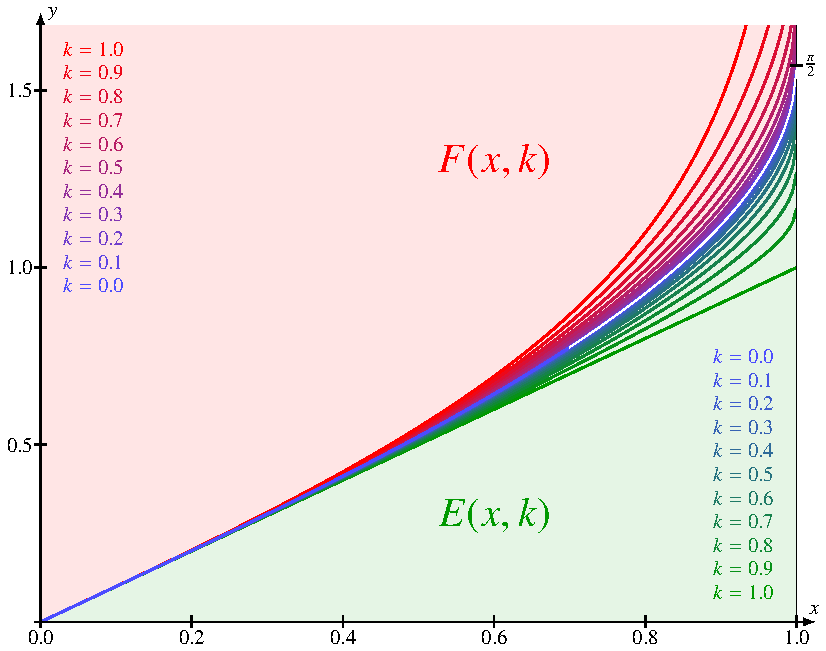
\includegraphics{chapters/110-elliptisch/images/unvollstaendig.pdf}
\caption{Unvollständige elliptische Integrale $F(x,k)$ und $E(x,k)$
für verschiedene Werte des Parameters $k$.
Für $k=0$ stimmen die Integrale erster und zweiter Art überein,
$F(x,0)=E(x,0)$.
\label{buch:elliptisch:fig:unvollstaendigeintegrale}}
\end{figure}
Wegen $k<1$ sind alle drei Integranden als reelle Funktionen nicht
mehr definiert, wenn $|x|>1$ ist.
Die Abbildung~\ref{buch:elliptisch:fig:unvollstaendigeintegrale}
zeigt Graphen der unvollständigen elliptischen Integrale für verschiedene
Werte des Parameters.

%
% Symmetrieeigenschaften
%
\subsubsection{Symmetrieeigenschaften}
Die Integranden aller drei unvollständigen elliptischen Integrale
sind gerade Funktionen der reellen Variablen $t$.
Die Funktionen $F(x,k)$, $E(x,k)$ und $\Pi(n,x,k)$ sind daher
ungeraden Funktionen von $x$.

%
% Elliptische Integrale als komplexe Funktionen
%
\subsubsection{Elliptische Integrale als komplexe Funktionen}
Die unvollständigen elliptischen Integrale $F(x,k)$, $F(x,k)$ und $\Pi(n,x,k)$
in Jacobi-Form lassen sich auch für komplexe Argumente interpretieren.
Dazu muss für die Berechnung des Integrals ein Pfad in der komplexen
Ebene gewählt werden, der die Singulariätten des Integranden vermeidet.

Die Faktoren, die in den Integranden der unvollständigen elliptischen
Integrale vorkommen, haben Nullstellen bei $\pm1$, $\pm1/k$ und
$\pm 1/\sqrt{n}$

% XXX Additionstheoreme \\
% XXX Parameterkonventionen \\

%
% Wertebereich
%
\subsubsection{Wertebereich}
\label{buch:elliptische:subsubsection:wertebereich}
Die unvollständigen elliptischen Integrale betrachtet als reelle Funktionen
haben nur positive relle Werte.
Zum Beispiel nimmt das unvollständige elliptische Integral erster Art
$F(k,x)$ nur Werte zwischen $0$ und $K(k)$ an.
Wenn komplexe Werte zulässig sind, kann man das Integral auch über die 
Singularitäten bei $\pm 1$ und $\pm 1/k$ hinweg ausführen, erhält
dabe aber möglicherweise komplexe Werte, weil die Radikanden in den
Integralen negativ werden.
Die Schwierigkeit dabei ist, dass die Quadratwurzel nicht eindeutig ist.
Welcher Wert der im Zusammenhang richtige ist, hängt davon ab, wie wir
dorthin kommen.

Die reelle Achse teilt den Definitionsbereich der unvollständigen
elliptischen Integrale in die obere und die untere Halbebene.
die Werte für reelle Argument beschreiben daher den Rand der Wertebereichs
für Argumente in der oberen bzw.~untere Halbebene.
Indem wir die Werte der elliptischen Integrale für reelle Argumente
berechnen, können wir daher den Rand des Wertebereichs ermitteln.

Im folgenden diskutieren wir nur das elliptische Integral erster Art,
die anderen können in der gleichen Art behandelt werden.
Für Argumentwerte $x$ im Interval $[0,1]$ ist $F(k,x)\in\mathbb{R}$.
An der Stelle $x=1$ wechselt der Faktor $(1-t^2)$ im Nenner das
Vorzeichen, der Integrand wird negativ.
Für Argumente zwischen $1$ und $1/k$ ist bleibt der Integrand negativ,
es muss also ein Wert der Quadratwurzel gewählt werden.
Beide Vorzeichen von
\begin{equation}
\frac{1}{\sqrt{(1-t^2)(1-k^2t^2)}}
=
\frac{\pm i}{\sqrt{(t^2-1)(1-k^2t^2)}}
\label{buch:elliptisch:eqn:imaginaerintegrand}
\end{equation}
sind möglich.
Doch welche Wahl ist die ``richtige''?

Dazu betrachten wir die Argument $z=x+i\varepsilon$ auf einer Geraden
parallel zur reellen Achse des Definitionsbereichs und in der oberen
Halbebene.
Da eine holomorphe Funktion die Orientierung erhält und weil das
Interval $[0,1]$ auf die reelle Achse abgebildet wird, müssen wir das
Vorzeichen der Wurzel so wählen, dass die Werte der Wurzel ebenfalls
in der oberen Halbebene liegen.
Die ``richtige'' Wahl der Wurzel von 
\[
1-z^2 = 1-x^2-2i\varepsilon x + \varepsilon^2
\]
erfüllt zwei Bedingungen.
\begin{enumerate}
\item
Für nicht zu grosse Werte von $x$ muss der Wert in der oberen
Halbebene liegen.
Für solche Werte von $x$ ist der Realteil $1-x^2+\varepsilon^2>0$ und
der Imaginärteil $-2\varepsilon x<0$.
Für die Wurzel muss man also das Argument von $1-z^2$ als Winkel zwischen
$3\pi2$ und $2\pi$ wählen und für die Wurzel durch zwei teilen.
\item
Der Realteil von $1-z^2$ wechsel das Vorzeichen, wenn
$x=\sqrt{1+\varepsilon^2}$, der Imaginärteil bleibt dabei negativ.
Das Argument ändert von einem Winkel nahe bei aber kleiner als $2\pi$
zu einem Winkel nahe bei aber grösser als $\pi$.
Als Wurzel muss daher jene verwendet werden, deren Argument in der
Nähe von $\frac{\pi}2$ liegt.
\end{enumerate}
Aus diesem Argument kann man ableiten, dass für die Berandung des
Bildes der oberen Halbebene zwischen $1$ und $1/k$ das positive
Zeichen in~\eqref{buch:elliptisch:eqn:imaginaerintegrand}
gewählt werden muss.

Die anderen Singularitäten auf der reellen Achse können analog
behandelt werden und es folgt, dass das Bild der oberen Halbebene
ein Rechteck in der oberen Halbebene ist
(Abbildung~\ref{buch:elliptisch:fig:rechteck}).
Die Ecken auf der reellen Achse liegen bei den reellen Koordinaten
\[
\pm F(1,k)
=
\pm\int_0^1\frac{dt}{\sqrt{(1-t^2)(1-k^2t^2)}}
=
\pm K(k).
\]
Für die Höhe muss das Integral
\begin{equation}
l({\textstyle\frac{1}{k}})=\int_1^{\frac1{k}}
\frac{dt}{\sqrt{(t^2-1)(1-k^2t^2)}}
\label{buch:elliptisch:eqn:hoeheintegral}
\end{equation}
ausgewertet werden.

%
% Komplementärmodul
%
\subsubsection{Komplementärmodul}
Im vorangegangen Abschnitt wurde gezeigt, dass der Wertebereicht des
unvollständigen elliptischen Integrals der ersten Art als komplexe
Funktion ein Rechteck ist.
Die obere Halbebene wird auf Rechteck der Breite $2K(k)$ abgebildet,
für die Höhe des Rechtecks muss das
Integral~\eqref{buch:elliptisch:eqn:hoeheintegral} ausgewertet werden.
Das Integral läuft von $t=1$ bis $t=1/k$, wir möchten daraus ein
elliptisches Integral machen, dessen Integrationsinterval bei $0$
beginnt.
Dazu verwenden wir die Variablentransformation
\[
t = \frac{1}{\sqrt{1-k'^2y^2}},
\]
die für $y=0$ den Wert $1$ ergibt, für $y=1$ aber $1/\sqrt{1-k'^2}$.
Damit das richtige Integrationsintervall entsteht, muss $k'$ so gewählt
werden, dass $1-k'^2=k^2$ ist.

\begin{definition}
Ist $0\le k\le 1$ der Modul eines elliptischen Integrals, dann heisst
$k' = \sqrt{1-k^2}$ der {\em Komplementärmodul} oder {\em Komplement
des Moduls}. Es ist $k^2+k'^2=1$.
\end{definition}

Mit der Ableitung
\[
\frac{dt}{dy}
=
\frac{k'^2 y}{(1-k'^2y^2)^{\frac32}}
\]
der Substitution
wird das Integral~\eqref{buch:elliptisch:eqn:hoeheintegral} mit der
oberen Grenze $x$ zu einem Integral mit oberer Grenze
\[
x^2 = \frac{1}{1-k'^2y_0^2}
\quad\Rightarrow\quad
y_0^2 = \frac{1}{k'^2}\biggl(1-\frac{1}{x^2}\biggr)
\quad\Rightarrow\quad
y_0=\frac{1}{k'}\sqrt{1-\frac{1}{x^2}}
\]
jetzt zu
\begin{align*}
l(x)
&=
\int_0^{y_0}
\frac{1}{\sqrt{\frac{1}{1-k'^2y^2}-1}}
\cdot
\frac{1}{\sqrt{1-\frac{k^2}{1-k'^2y^2}}}
\cdot
\frac{k'^2y}{\sqrt{1-k'^2y^2}}
\cdot
\frac{1}{1-k'^2y^2}
\,dy
\\
&=
\int_0^{y_0}
\frac{\sqrt{1-k'^2y^2}}{\sqrt{k'^2y^2}}
\cdot
\frac{1}{\sqrt{1-k^2 -k'^2y^2}}
\cdot
\frac{k'^2y}{1-k'^2y^2}
\,dy
\\
&=
\int_0^{y_0}
\sqrt{1-k'^2y^2}
\cdot
\frac{1}{k'\sqrt{1-y^2}}
\cdot
\frac{k'}{1-k'^2y^2}
\,dy
\\
&=
\int_0^{y_0} \frac{dy}{\sqrt{(1-y^2)(1-k'^2y^2)}}
=
F(y_0,k')
\end{align*}
Die gesuchte Höhe des Rechtecks ergibt sich für die obere Grenze $\frac1k$.
In diesem Fall ist
\[
y_0
=
\frac{1}{k'}\sqrt{1-k^2} = 1
\]
und das unvollständig elliptische Integral wird zum vollständigen
elliptischen Integral $K(k')$.
Die Höhe des Rechtecks des Wertebereichs der oberen Halbebene ist
als der Wert des vollständigen elliptischen Integrals erster Art
für den Komplementärmodul.
Das Bild der komplexen Ebene unter der Abbildung gegeben durch das
unvollständige elliptische Integral zweiter Art ist symmetrisch um
den Nullpunkt und hat Breite $2K(k)$ und Höhe $2K(k')$.

\begin{figure}
\centering
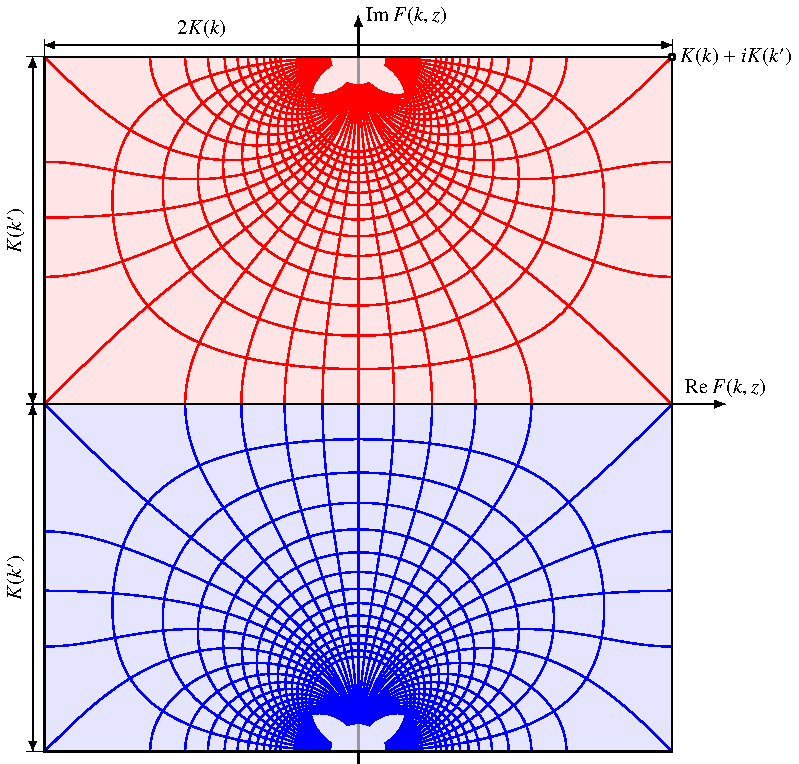
\includegraphics{chapters/110-elliptisch/images/rechteck.pdf}
\caption{Der Wertebereich der Funktion $F(k,z)$ ist ein Rechteck
der Breite $2K(k)$ und $2K(k')$.
Die obere Halbebene wird in das rote Rechteck abgebildet, die unter
in das blaue.
\label{buch:elliptisch:fig:rechteck}}
\end{figure}

%
% Reelle Argument > 1/k
%
\subsubsection{Reelle Argument $> 1/k$}
Für Argument $x> 1/k$ sind beide Faktoren im Integranden des 
unvollständigen elliptischen Integrals negativ, das Integral kann
daher wieder als gewöhnliches reelles Integral berechnet werden,
es sollte sich daher auch auf das unvollständige elliptische Integral
erster Art zurückführen lassen.

Da wir bereits wissen, dass 
\[
\lim_{x\to\infty} F(x,k) = iK(k'),
\]
können wir $F(x,k)$ auch als
\[
F(x,k)
=
iK(k')
-
\int_x^\infty \frac{dt}{\sqrt{(1-t^2)(1-k^2t^2)}}
\]
berechnen.
Dazu werden wir die Variablentransformation
\[
y=\frac{1}{kt}\quad\Leftrightarrow\quad t=\frac{1}{ky}
\qquad\text{mit}\qquad
\frac{dt}{dy} = -\frac{1}{ky^2}
\]
auf das Integral an und erhalten
\begin{align*}
\int_x^\infty \frac{dt}{\sqrt{(1-t^2)(1-k^2t^2)}}
&=
-\int_{\frac1{kx}}^0 \frac{dy}{ky^2\sqrt{(1-1/(ky)^2)(1-1/y^2)}}
\\
&=
\int_0^{\frac{1}{kx}} \frac{dy}{\sqrt{(k^2y^2-1)(y^2-1)}}
=
F\biggl(\frac{1}{kx},k\biggr).
\end{align*}
Dies ist das gesuchte unvollständige elliptische Integral erster Art.
Insbesondere halten wir noch die Formel
\[
F(x,k) = iK(k') - F\biggl(\frac1{kx},k\biggr)
\qquad\text{für $x>\frac1k$}
\]
für die Werte des elliptischen Integrals erster Art für grosse Argumentwerte
fest.

%
% AGM und Berechnung von F(x,k)
%
\subsubsection{Berechnung von $F(x,k)$ mit dem arithmetisch-geometrischen Mittel\label{buch:elliptisch:subsubection:berechnung-fxk-agm}}
Wie das vollständige elliptische Integral $K(k)$ kann auch das  
unvollständige elliptische Integral
\begin{align*}
F(x,k)
&=
\int_0^x \frac{d\xi}{\sqrt{(1-\xi^2)(1-k^{\prime 2}\xi^2)}}
=
\int_0^{\varphi}
\frac{dt}{\sqrt{1-k^2 \sin^2 t}}
\\
&=
a
\int_0^{\varphi} \frac{dt}{a^2 \cos^2 t + b^2 \sin^2 t}
\qquad\text{mit $k=b/a$}
\end{align*}
mit dem arithmetisch-geometrischen Mittel berechnet werden.
Dazu muss die Substitution
\eqref{buch:elliptisch:agm:subst}
verwendet werden, um auch den Winkel $\varphi_1$ zu berechnen.
Dazu muss \eqref{buch:elliptisch:agm:subst} nach $x_1=\sin t_1$ 
aufgelöst werden.
Durch Multiplikation mit dem Nenner erhält man mit der Abkürzung
$x=\sin t$ und $x_1=\sin t_1$  die quadratische Gleichung
\[
(a-b)x x_1
-
2ax_1
(a+b)x 
=
0,
\]
mit der Lösung
\begin{equation}
x_1 
=
\frac{a-\sqrt{a^2-(a^2-b^2)x^2}}{(a-b)x}.
\label{buch:elliptisch:unvollstagm:xrek}
\end{equation}
Der Algorithmus zur Berechnung des arithmetisch-geometrischen Mittels
muss daher verallgemeinert werden zu
\begin{equation}
\left.
\begin{aligned}
a_{n+1} &= \frac{a_n+b_n}2,  &\qquad a_0 &= a
\\
b_{n+1} &= \sqrt{a_nb_n},    & b_0 &= b
\\
x_{n+1} &= \frac{a_n-\sqrt{a_n^2-(a_n^2-b_n^2)x_n^2}}{(a_n-b_n)x_n}, & x_0 &= x
\end{aligned}
\quad
\right\}
\label{buch:elliptisch:unvollstagm:rek}
\end{equation}
Die Folge $x_n$ konvergiert gegen einen Wert $x_{\infty} = \lim_{n\to\infty} x_n$.
Der Wert des unvollständigen elliptischen Integrals ist dann der Grenzwert
\[
F(x,k)
=
\lim_{n\to\infty}
\frac{\arcsin x_n}{M(a_n,b_n)}
=
\frac{\arcsin x_{\infty}}{M(1,\sqrt{1-k^2})}.
\]

In dieser Form ist die Berechnung allerdings nicht praktisch durchführbar.
Das Problem ist, dass die Differenz $a_n-b_n$, die in 
\eqref{buch:elliptisch:unvollstagm:rek}
im Nenner vorkommt, sehr schnell gegen Null geht.
Ausserdem ist die Quadratwurzel im Zähler fast gleich gross wie
$a_n$, was zu Auslöschung und damit ungenauen Resultaten führt.
\label{buch:elliptisch:agm:ellintegral-stabilitaet}

Eine Möglichkeit, das Problem zu entschärfen, ist, die Rekursionsformel
nach $\varepsilon = a-b$ zu entwickeln.
Mit $a+b=2a+\varepsilon$ kann man $b$ aus der Formel elimineren und erhält
mit Hilfe der binomischen Reihe
\begin{align*}
x_1
&=
\frac{a}{x\varepsilon}
\left(1-\sqrt{1-\varepsilon(2a-\varepsilon)x^2/a^2}\right)
\\
&=
\frac{a}{x\varepsilon}
\biggl(
1-\sum_{k=0}^\infty
(-1)^k
\frac{(\frac12)_k}{k!} \varepsilon^k(2a-\varepsilon)^k\frac{x^{2k}}{a^{2k}}
\biggr)
\\
&=
\sum_{k=1}^\infty
(-1)^{k-1} 
\frac{(\frac12)_k}{k!} \varepsilon^{k-1}(2a-\varepsilon)^k\frac{x^{2k-1}}{a^{2k-1}}
\\
&=
\frac{\frac12}{1!}(2a-\varepsilon)\frac{x}{a}
-
\frac{\frac12\cdot(\frac12-1)}{2!}\varepsilon(2a-\varepsilon)^2\frac{x^3}{a^3}
+
\frac{\frac12\cdot(\frac12-1)(\frac12-2)}{3!}\varepsilon^2(2a-\varepsilon)^3\frac{x^5}{a^5}
-
\dots
\\
&=
x\biggl(1-\frac{\varepsilon}{2a}\biggr)
\biggl(
1
-
\frac{\frac12-1}{2!}\varepsilon(2a-\varepsilon)\frac{x^2}{a^2}
+
\frac{(\frac12-1)(\frac12-2)}{3!}\varepsilon^2(2a-\varepsilon)^2\frac{x^4}{a^4}
-
\dots
\biggr)
\\
&=
x\biggl(1-\frac{\varepsilon}{2a}\biggr)
\cdot
\mathstrut_2F_1\biggl(
\begin{matrix}-\frac12,1\\2\end{matrix};-\varepsilon(2a-\varepsilon)\frac{x^2}{a^2}
\biggr).
\end{align*}
Diese Form ist wesentlich besser, aber leider kann es bei der numerischen
Rechnung passieren, dass $\varepsilon < 0$ wird.

%\subsection{Potenzreihe}
%XXX Potenzreihen \\
%XXX Als hypergeometrische Funktionen \url{https://www.youtube.com/watch?v=j0t1yWrvKmE} \\
%XXX Berechnung mit der Landen-Transformation https://en.wikipedia.org/wiki/Landen%27s_transformation
